\documentclass[10pt,twocolumn]{article} 

% required packages for Oxy Comps style
\usepackage{oxycomps} % the main oxycomps style file
\usepackage{times} % use Times as the default font
\usepackage[style=numeric,sorting=nyt]{biblatex} % format the bibliography nicely

\usepackage{amsfonts} % provides many math symbols/fonts
\usepackage{listings} % provides the lstlisting environment
\usepackage{amssymb} % provides many math symbols/fonts
\usepackage{graphicx} % allows insertion of grpahics
\usepackage{hyperref} % creates links within the page and to URLs
\usepackage{url} % formats URLs properly
\usepackage{verbatim} % provides the comment environment
\usepackage{xpatch} % used to patch \textcite

\bibliography{references}
\DeclareNameAlias{default}{last-first}

\xpatchbibmacro{textcite}
  {\printnames{labelname}}
  {\printnames{labelname} (\printfield{year})}
  {}
  {}

\pdfinfo{
    /Title (Writing Your Oxy CS Comps Paper in LaTeX)
    /Author (Maryo Botros)
}

\title{SLAM}

\author{Maryo Botros}
\affiliation{Occidental College}
\email{mbotros@oxy.edu}

\begin{document}

\maketitle

\begin{abstract}
    Abstract
\end{abstract}

\section{Problem Context}

Robotics boasts a significant benefit in accomplishing repeatable, tedious, or menial tasks at high effieciencies and with great resource utilization. Robots can increase relative productivity and decrease resource and energy consumption by multiple orders of magnitude for processes. They can also offer high-precision with limited human oversight for the tasks they are designed for. The real benefit of robotics comes in where robotics can serve as a substitute for human labor, more specifically, human labor that can potentially put humans in harm's way and some of the best robots for accomplishing this task are vehicles that can navigate autonomously. An example of one of these tasks includes using the robot to enter a building on fire to search for and potentially rescue people. Another application can be for military applications, such as reconnaissance. These are just two of the many possible applications of autonomous vehicles. These robots are very useful, but getting them to accomplish the task of being autonomous does not come easily.

The problem is that getting a robot to navigate any environment is challenging and is rooted in uncertainty. There are two things a robot must be able to do to autonomously navigate. It must understand the map of its environment, which is known as mapping. It must also know where it is on that map, which is known as localization. The problem is that in order for the robot to know where it is on the map, it must first understand the map, but in order for it to understand the map, it must first understand where it is on the map. This poses a major challenge because there are conflicting dependent conditions. The solution to this problem is doing both the mapping and the localization at the same time and this process is known as SLAM. SLAM means simultaneous localization and mapping and it's the method for getting a robot to autonomously navigate its environment. SLAM is still an open problem and new ways of solving the problems of navigation are still being researched constantly.

    

    


\section{Technical Background}

A few of the problems involved with navigation that will be covered in this project are localization, searching for the goal location, planning a path to the goal location, covering an entire area, and SLAM.

One of the ways localization is accomplished for robots is using odometry or the distance the robot has traveled. Shaft encoders are the sensors used for odometry. One problem with this however is that the farther the robot has traveled, the more inaccurate the odometry will be because measurements of the physical environment are unavoidable.

Search and path planning involves finding a path from the robot’s current location, to the destination. Two things that the robot would have to know to do this are what the map looks like as well as where it is on that map (localization). It must know both of these within a common frame of reference. There are typically many different paths for getting to the destination from the starting point. Graphs with nodes and lines are usually used for modeling a map. The criterion for the optimal path can be safety or distance for example and finding the optimal path may require searching all paths. A maze is one of the best ways of testing a robot’s ability to get to a goal location. One of the methods for solving a maze can be programming the robot to follow one of the walls of the maze. This method will work but it is the naive solution and is not the most efficient as it can take a long time, depending on the complexity of the maze. A much more optimal solution for solving a maze is by using a depth-first search approach, where the robot will keep track of each path option in the maze as a node and it will go down all the nodes along a single path first before it backtracks and then goes along a different path until it has found the exit to the maze. The way this would be executed is by using a graph data structure, like the one in Figure 1. The graph is a good model for the maze. Each junction in the maze is recorded as a node in the graph model. There are several other algorithms besides the depth-first search for navigating the maze, such as a breadth-first search, but this is one of the most efficient solutions.

Coverage is a problem that certain robots such as robot vacuums need to be able to efficiently solve. If the robot has a map available to it, the problem of coverage becomes a lot easier. In this case, the robot would need all navigable spaces on the map until the whole map is covered, or the robot has accomplished its designated goal, such as searching for an object or reaching a destination. If the robot does not have a map available, there are certain heuristics it can follow such as following a continuous boundary like a wall. 

SLAM is a difficult problem because it requires the robot to do two ongoing processes. One thing that makes SLAM difficult is the data association problem, or basically, the problem that certain locations on the map may look similar, which leads to ambiguity while the robot is navigating. When the robot is constructing a map, if it sees a particular chair at one location and then sees a similar chair at a different location, it would have a hard time distinguishing the two.

\begin{figure}
    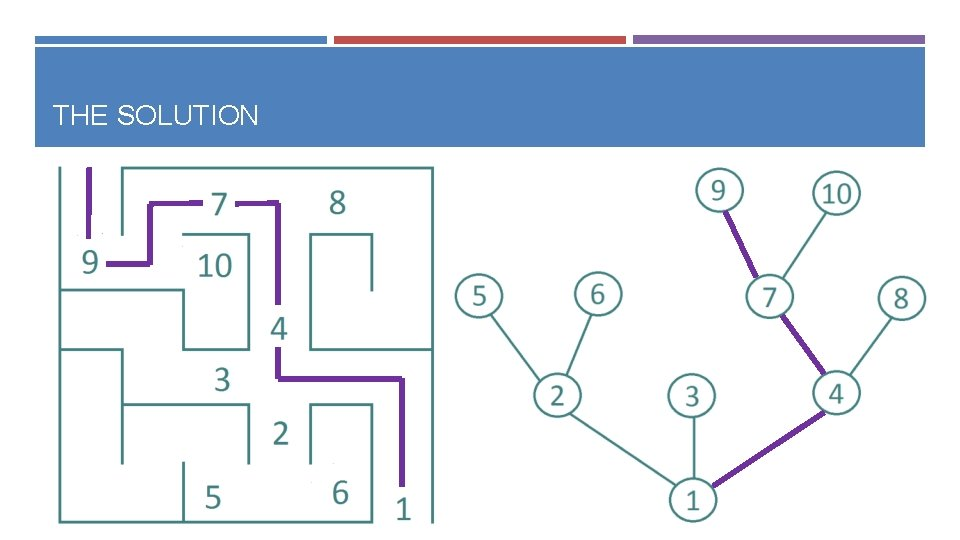
\includegraphics[width=\linewidth]{graph.jpg}
    \caption{Maze and graph}
    \label{fig1}
  \end{figure}
  
Beyond the basic syntax, much of learning LaTeX is learning the different commands and environments that exist.
For example, text can be made \textbf{bold} with \texttt{\textbackslash textbf}, \textit{italic} with \texttt{\textbackslash textit}, and \texttt{monospaced} with \texttt{\textbackslash texttt} (the \texttt{tt} stands for for ``teletype'').
Single dollar signs denote inline equations, so \texttt{\$E = mc\textasciicircum 2\$} will be rendered as $E = mc^2$.
Double dollar signs will render the equation in display mode, which we can see with the quadratic formula:
$$\frac{{-b \pm \sqrt {b^2 - 4ac} }}{{2a}}$$
There are also a handful of common environments: \texttt{itemize} for bulletpoint lists, \texttt{enumerate} for numbered lists, \texttt{figure} for figures, \texttt{tabular} for tables, and \texttt{lstlisting} for code listings.
This covers the most frequently used commands, but as you might have already inferred, LaTeX is a vast and deep system, and can easily be overwhelming.
We recommended following the \citetitle{Overleaf2021LearnLaTeXIn} tutorial \cite{Overleaf2021LearnLaTeXIn}, and examining and playing with the source of this document, to gain working proficiency with LaTeX.

One final note on writing in LaTeX.
Since LaTeX is only a markup language, the source files must be compiled into a viewable form, most commonly into a PDF file.
The source of this document is made up of several files, each with its own purpose:
\begin{itemize}
    \item \texttt{template.tex} - The main LaTeX file containing the contents of the document.
    \item \texttt{oxycomps.sty} - A style file with settings for what the document should look like.
    \item \texttt{references.bib} - A list of bibliography items.
    \item Other files containing images, build instructions, etc.
\end{itemize}
Manual compilation of these files is somewhat esoteric, as it requires multiple uses of the \texttt{pdflatex} and \texttt{biblatex} commands.
Instead, it is much easier to use tools such as \texttt{latexmk} (in the terminal) or Overleaf (online) for compilation.
We have also provided a \texttt{Makefile} which will automatically update the document as necessary; the use of makefiles is beyond the scope of this document, but see \textcite{Lambert2021MakefileTutorial}.

\begin{comment}

\begin{figure}[]
    \begin{center}
        \includegraphics[width=\linewidth]{figure.pdf}
    \end{center}
    \caption{
        Figure caption.
        To get a figure to span two columns, use the {\tt figure*} environment rather than {\tt figure}.
    }
    \label{figure1}
\end{figure}

\begin{quote}
    Lorem ipsum dolor sit amet, consectetur adipiscing elit.
    Mauris pellentesque est nec nunc fringilla, a finibus nisl tempor.
    Sed semper est massa, eget pulvinar neque posuere id.
    Ut mauris tellus. 
\end{quote}

\begin{lstlisting}[language=Python]
def hello():
    print('hello, world!')
\end{lstlisting}

\end{comment}

\begin{comment}
No definition citations, unless the term itself is in dispute
Separate problem background from technical background
    Unclear if games and apps require much technical background
    The general structure of the framework might be better suited for the Architecture Overview section
        Eg. Flask uses decorators to associate functions with URLs
        Eg. Unity has scripts associated with objects and specific triggers, such as walking into an area, pressing a button, etc.
    Maybe a better name is "algorithmic background"?
        Should explore what does and doesn't count
            All ML counts
            App and game frameworks do not
        Framework vs. library?
            I like the idea of [inversion of control](https://martinfowler.com/bliki/InversionOfControl.html), but that may be too abstract for students to understand
        Heuristic: is understanding that system necessary to understand the results?
            Ie. How Flask or Unity works doesn't influence whether the app/game is useful/fun/engaging
            But how (say) linear regression works is highly relevant for why the results match/don't match the actual values
\end{comment}

\section{Prior Work}

\subsection{Goals}

\subsection{Audience}

\subsection{Requirements}

\section{Sections of the Oxy CS Comps Paper}

\subsection{Introduction and Background}


\subsection{Prior Work}

\subsection{Methods}

\subsection{Evaluation}

\subsection{Ethical Considerations}

\subsection{Limitations, Future Work, and Conclusion}

\subsection{Appendices}

\section{Conclusion}

\printbibliography 

\end{document}
